\chapter{Case study: FRP in real-time data flows} % (fold)
\label{sec:uitwerking}

In this chapter a real-time chat application is developed and analyzed. The chat application is implemented twice in different programming styles. The first implementation uses FRP for all application logic and Cycle.js to render this to the Document Object Model. The second implementation uses imperative programming for all application logic and JQuery for DOM manipulation.

The backend implementation is the same for both frontend implementations. Real-time communication between server and client is implemented using WebSockets. WebSockets was chosen over HTTP long polling because long polling does not implement a full-duplex communication channel. WebSockets were chosen over WebRTC data channels because of browser support and maturity of the protocol. Furthermore WebRTC is primarily meant for P2P applications and is cumbersome to implement in a client-server application model.

The source code of this application is open source and is available on GitHub \cite{chat-code}. Excerpts from the source code will be included throughout this chapter to explain implementation details. 

\section{Interface}

The application features a very simple interface (see figure~\ref{figure:chat}). Users can enter their name and a message in the text inputs in the bottom bar. They can then click send to send a new message over the WebSocket. The server will then broadcast this message to all other clients connected to the WebSocket. 

On the frontend the messages are displayed with an avatar next to them that is automatically generated from the username of the sender. The side the messages are rendered on is dependent on whether the current user is equal to the sender of the message. A user's own messages will appear on the right and messages from other people will appear on the left.

\begin{figure}[H]
	\centering
	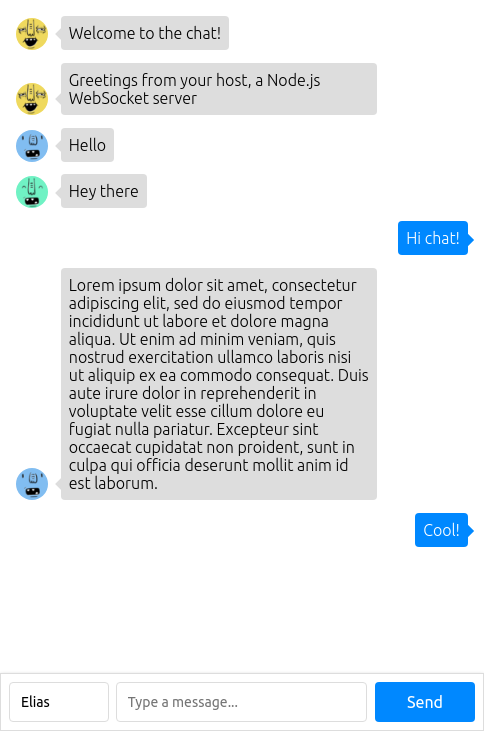
\includegraphics[width=0.6\textwidth]{chat}
	\caption{The chat application interface}
	\label{figure:chat}
\end{figure}

\section{Backend}

\subsection{Implementation}

The backend is implemented in Node.js. It makes use of the Express framework to set up an HTTP server and host the static files from the frontend. The WebSocket implementation used is µWebSockets. µWebSockets is a lightweight WebSocket implementation written in C++ with simplicity, performance and scalability as its main objectives \cite{uws}.

µWebSockets was chosen because of its simplicity and performance. This application is meant to be a very minimal implementation of a chat application and as a result it does not need any extra features on top of the WebSocket protocol. Socket.IO or other popular WebSocket libraries would have been overkill for this application as it does not need any of the extra features it provides.

Messages are not persisted on the server because it would add extra dependencies and potential performance bottlenecks. This case study is focused on the comparison of FRP and imperative programming for the web. As a result it was attempted to add as little dependencies as possible to focus on that comparison.

\subsection{Functionality}

The backend sets up the WebSocket using µWebSockets and listens for connections. When a client connects to the WebSocket the server sends out a welcome message. When a client sends a message over the WebSocket the server will broadcast this message to all clients that are currently connected.

\section{Frontend with FRP}
\label{sec:imp-frp}

\subsection{Choice of technologies}

\subsubsection{FRP library}

RxJS is used as the FRP library for this application. This choice is made mainly because of the popularity of the library. ReactiveX is a very mature cross-language FRP library with big companies like Microsoft and Netflix backing it and using it in their own applications \cite{rx}. The JavaScript version of ReactiveX (RxJS) is currently the most popular FRP library for JavaScript by a large margin. The npm installation statistics support this statement \cite{rx-npm}\cite{most-npm}\cite{xs-npm}.

Xstream and most.js were also considered. Both these FRP libraries feature better performance than RxJS and are only a fraction of the size \cite{rx-npm}\cite{most-npm}\cite{xs-npm}. But ultimately the performance and bundle size of this application is not the priority. Using RxJS has the advantage of more people being familiar with its concepts and operators.

\subsubsection{DOM abstraction}

For a DOM abstraction various frameworks and libraries are considered. Since the objective is to use FRP in the application, frameworks that play nice with FRP have the advantage. Angular is the first framework that comes to mind in this category. Angular has built-in support for observables and even uses RxJS internally for its core API's. But because of the size and complexity of Angular there is too much overhead for this application. This application is meant to be as minimal as possible and Angular does not fit the bill in that department.

Cycle.js is the next framework to be considered. Cycle.js is a functional and reactive JavaScript framework for predictable code \cite{cycle} written by André Staltz who is also a core contributor to RxJS and the author of xstream \cite{staltz}\cite{xs-npm}. Cycle.js features a very minimal API and allows the programmer to see the application as a pure function. To use Cycle.js the programmer has to only import one function \code{run()}. This makes code easy to understand for newcomers since there are no new framework API's to learn. Cycle.js is also FRP library agnostic and thus allows the programmer to use their library of choice.

Because of its minimal API and very functional architecture Cycle.js was chosen as the DOM abstraction for this application. The architecture used in Cycle.js is further explained in  section~\ref{sec:arch}.


\subsection{Architecture}
\label{sec:arch}

Cycle.js lets the developer see the app as a pure function. This \code{main()} function takes source streams as an argument and returns sink streams. Figure~\ref{figure:cycle} shows a diagram of how this architecture works in practice.

\begin{figure}[H]
	\centering
	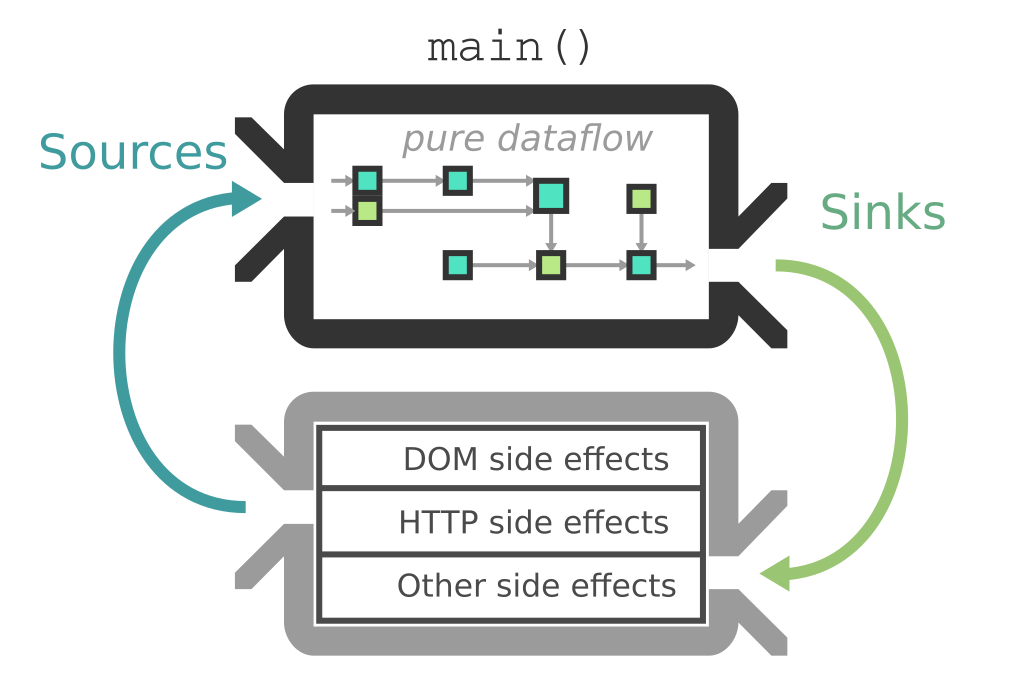
\includegraphics[width=0.8\textwidth]{cycle}
	\caption{Cycle.js application architecture \cite{cycle}}
	\label{figure:cycle}
\end{figure}

The bottom function shown in figure~\ref{figure:cycle} is called a driver. Drivers handle side effects towards various outputs such as the DOM. Drivers take sinks as an argument and return sources for the main function to use \cite{cycle-drivers}. Driver functions can be seen as the inverse of the \code{main()} function. Cycle.js provides a few basic drivers for the DOM and for HTTP requests. Cycle.js is very extensible \cite{cycle-drivers} and as a result other drivers written by the community can be found on open source platforms.

\begin{figure}[H]
	\centering
	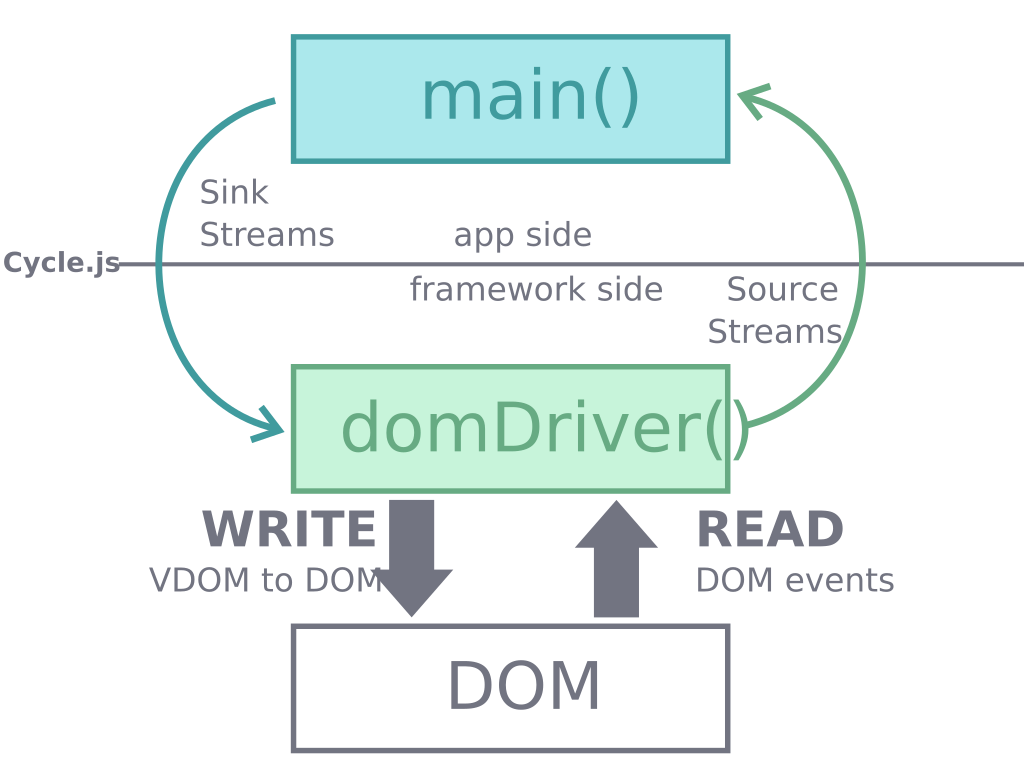
\includegraphics[width=0.7\textwidth]{driver}
	\caption{Cycle.js DOM driver diagram \cite{cycle-drivers}}
	\label{figure:driver}
\end{figure}

The diagram shown in figure~\ref{figure:driver} is an example of a Cycle.js driver. It represents the built-in DOM driver. This driver handles writing DOM changes from the sink stream and provides DOM elements and events in the source stream.

\subsubsection{Custom WebSocket driver}

For this project a custom driver was developed to set the WebSocket up as a source and a sink stream. The driver is available as a package on npm \cite{driver-npm} so that it can be used by other users of Cycle.js. The source code is open source and is available on GitHub \cite{driver-github}.

The driver is a wrapper around the WebSocketSubject object provided by RxJS \cite{ws-subject}. Internally the driver acts as an adapter that forwards the messages from the sink stream to the WebSocketSubject. The driver returns the WebSocketSubject as a whole as a source stream, that way the developer has full control over it in the \code{main()} function. Special attention was given to ensure that the driver is also compatible with other FRP libraries such as xstream and Most.js.

\subsection{Implementation}

When developing an application with the concept of source and sink streams the developer first defines the input streams needed for the application. These input streams can be user input, a real-time database etc.

In the case of this application these input streams will be inputs from the user through DOM events and messages from the WebSocket. In the source code the input streams are defined as in listing~\ref{listing:input-streams}. The input streams are derived from the sources given as an argument to the Cycle.js \code{main()} function. In some cases the input streams might even be just a source without any mutation.

The \code{scan} operator on the WebSocket source collects all messages received up until this point in an array. The marble diagram in the comment on line 2 shows how this works in practice. \code{\{m\}} represents a single message object.

\begin{lstlisting}[caption=Definition and instantiation of the input streams,label=listing:input-streams]
const messages$ = ws.scan((acc, m) => [...acc, m], []);
// --[]--[{m}]--[{m}, {m}]--[{m}, {m}, {m}]-->
const formSubmit$ = DOM.select('#form').events('submit');
const senderInput$ = DOM.select('#sender').events('input');
const messageInput$ = DOM.select('#message').events('input');
\end{lstlisting}

After the input streams are defined the developer can think about what sinks (output streams) the application will output towards. In the case of web applications one sink that will always be used is the DOM. LocalStorage is an example of another output stream that some applications use. In the case of this application the used sinks are the DOM and the WebSocket.

Now that the sources and sinks are known all that is left to do is to combine and manipulate the input streams until they are in the required format for the sinks. Before writing any code it can be useful for the developer to make a dependency graph to see which output streams depend on which input streams. The dependency graph for this chat application is shown in figure~\ref{figure:chat-dep}.

\begin{figure}[H]
	\centering
	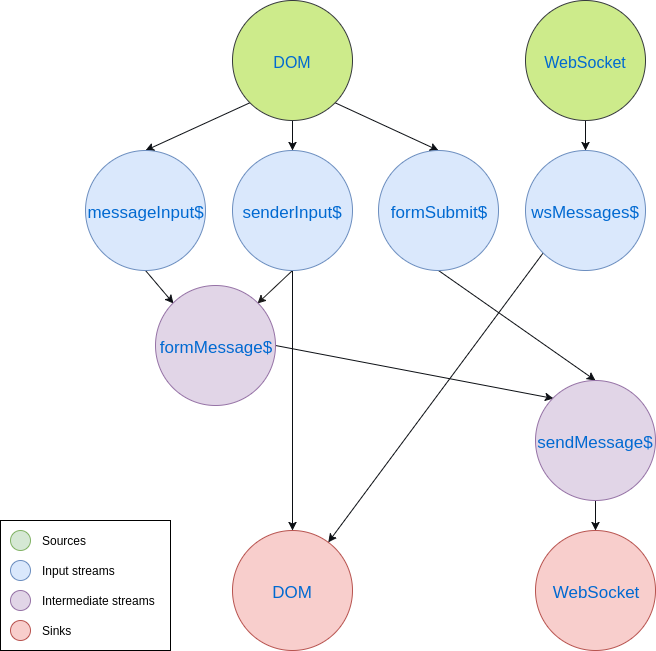
\includegraphics[width=0.7\textwidth]{chatdep}
	\caption{Dependency graph of the chat application}
	\label{figure:chat-dep}
\end{figure}

By using operators to mutate the input streams they are converted to the required format for the output streams. For the sake of readability intermediate streams are used. They are not required but are useful to make reasoning about the application easier. Finally the sinks are handled by the driver functions. The drivers will handle the I/O and side effects caused by the sinks. In the case of the chat application the DOM driver will rerender the DOM with the updated DOM and the WebSocket driver will send newly submitted messages over the WebSocket.

For elegant representation of the DOM in JavaScript JSX is used. JSX is not a templating language but rather a syntax extension to JavaScript \cite{jsx}. Because of this JSX comes with the full power of JavaScript. JSX was popularized by its use in React \cite{jsx}. In the code we provide the DOM sink as a stream of JSX objects (see listing~\ref{listing:jsx}).

\begin{lstlisting}[caption=Using JSX to define the DOM,label=listing:jsx]
function main({ DOM, ... }) { // sources in function argument
	...
	const vtree$ = Observable
		.combineLatest(wsMessages$.startWith([]), senderInput$.startWith(''))
		.map(([messages, me]) =>
			<div className="wrapper">
				<ul className="chat">
				{ messages && messages.map(m =>
					<li className={`chat__entry${me === m.sender ? ' chat__entry--mine' : ''}`}>
						<span className="chat__entry__message">{m.message}</span>
					</li>
				)}
				</ul>
			</div>
		);
		
	return { DOM: vtree$, ... }; // return sinks
}
\end{lstlisting}

In the code in listing~\ref{listing:jsx} the path towards the DOM sink in de dependency graph shown in figure~\ref{figure:chat-dep} can be recognized. The \code{wsMessages\$} and the \code{senderInput\$} streams are combined to render the current state of the application to the DOM. The \code{startWith} operators are used to define the initial state.

The JSX in listing~\ref{listing:jsx} in only an excerpt of the complete DOM. Only the logic to render the messages and determine if the message is from the sender is included. In JSX JavaScript language features are used to achieve this. To render the messages from an array of objects the \code{Array.map()} function is used. This function will map the individual messages to a JSX object. To determine if the current user is the sender of a particular message a ternary is used.

\section{Frontend with imperative programming}
\label{sec:imp-imp}

\subsection{Choice of technologies}

When developers create web applications with imperative programming they frequently use libraries such as JQuery as an abstraction over vanilla JavaScript. JQuery makes things like HTML document traversal and manipulation, event handling, animation, and Ajax simpler \cite{jquery}. While there are alternatives to JQuery like Dojo and Ext, JQuery has been and still is the most popular one by far. 

Monolithic abstractions over JavaScript like JQuery have been losing popularity in recent years because of smaller and more modular utility libraries such as lodash. New features and API's that are added to the JavaScript specification also diminish the need for JQuery. Last but not least more and more developers are migrating to more declarative frameworks and libraries to manipulate the DOM such as React.

For this application JQuery was chosen because it still sees the most usage compared to its competitors. React or Angular are not really options because they are not imperative programming frameworks.

\subsubsection{Templating language}

To render the application to the DOM it was decided to use a templating engine for convenience. Handlebars was chosen as the templating engine for the application. Handlebars provides some utility over Moustache which it is built upon. Handlebars is still a very minimal templating engine that is much lighter than popular competitors such as Pug and EJS. 

\subsection{Architecture}

The application uses a single \code{render()} function that is called whenever the application needs to rerender (see figure~\ref{figure:arch}). The application listens to events from the DOM and from the WebSocket. These events will then mutate objects that are stored in globally scoped mutable variables.

\begin{figure}[H]
	\centering
	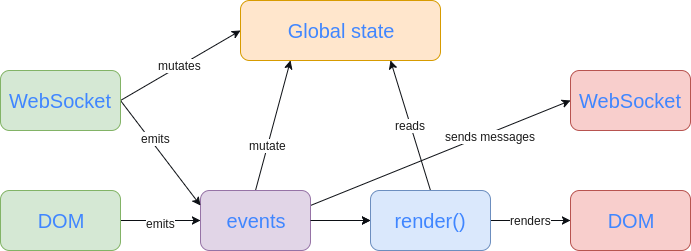
\includegraphics[width=\textwidth]{arch}
	\caption{Diagram of the imperative application architecture}
	\label{figure:arch}
\end{figure}

The event handlers from the \code{onmessage} event on the WebSocket and the \code{oninput} event from the sender input will call the \code{render()} function. Whenever the render function gets called it will read variables from the global state and rerender the application in the DOM. The onsubmit event from the message form will cause a new message to be sent over the WebSocket.

\subsection{Implementation}

This implementation uses event handlers to mutate a global state. This global state is instantiated as in listing~\ref{listing:state}.

\begin{lstlisting}[caption=The global variables that make up the application state,label=listing:state]
const template = Handlebars.compile(`
	<div class="wrapper">
		...
	</div>
`);

const messages = [];
let lastMessage = '';
let me = '';
\end{lstlisting}

The \code{messages} variable gets mutated from the \code{onmessage} event handler from the WebSocket. The \code{lastMessage} variable holds the last sent message so that it can be persisted as the input value after render. Lastly the me variable contains the current sender. This variable will be mutated by the \code{oninput}.

This application architecture is completely different from the FRP implementation. In that implementation the event streams were composed into an unidirectional dataflow (see figure~\ref{figure:chat-dep}). In this implementation event handlers are set up separately. They then all mutate global objects to communicate their data to other parts of the application. 

\subsubsection{Render function}
The \code{render()} function is implemented as shown in listing~\ref{listing:render}.
Internally the render function will compile the Handlebars template with the new data. To have the necessary data the render function first loops over the messages to check which ones are from the current user. Finally it replaces the previous version of the application in the DOM with the newly compiled Handlebars template.

\begin{lstlisting}[caption=Implementation of the render function,label=listing:render]
const render = () => {
	for (let i = 0; i < messages.length; i++) {
		const message = messages[i];
		message.isMine = message.sender === me;
	}
	const data = { messages, me, lastMessage };
	const htmlString = template(data);
	$('#app').html(htmlString);
	$('#sender').focus().val(me);
};
\end{lstlisting}

The last line of listing~\ref{listing:render} covers a corner case where the sender input loses focus while the user is typing because of the rerender. Another corner case that needed to be covered was initial render. Because the \code{render()} function only gets called from events the application would not render until an event occurs. To solve this the \code{render()} function also has to be called on load.

\section{Comparison}

In this chapter the two implementations from the section~\ref{sec:imp-frp} and section~\ref{sec:imp-imp} are compared with various metrics. First static analysis tools are used to analyze the application code. Second the performance of the two applications is compared. Finally some more subjective metrics like readability and extensibility are discussed.

\subsection{Static analysis}

\subsubsection{Bundle size}

\subsubsection{Code length}

\subsubsection{Code complexity}

\subsection{Performance}

\subsection{Readability}

\subsection{Extensibility}